
\section{OU process}
\begin{align}
\begin{cases}
dx_t = u_t dt+\xi dW_t'\\
du_t = -\gamma u_t dt+ \lambda dW_t
\end{cases}
\end{align}
The solutions are
\begin{align}
\begin{cases}
u_t &=u_{t-1}e^{-\gamma t} +\int_{0}^{t} \lambda e^{-\gamma (t-s)}dW_s,\\
x_t &=x_{t-1} +\frac{u_{t-1}}{\gamma}(1- e^{-\gamma t}) + \int_{0}^{t} \frac{\lambda}{\gamma}e^{\gamma  s} \left(1-e^{-\gamma t}\right)dW_s + \int_{0}^{t}\xi dW_s'.
\end{cases}
\end{align}
Therefore,
\begin{align*}
\begin{bmatrix} x_t \\ u_t \end{bmatrix} &\sim N\left(
\begin{bmatrix}\mu_t^{(x)} \\ \mu_t^{(u)}  \end{bmatrix} , 
\begin{bmatrix}
\sigma_t^{(x)2} & \rho_t\sigma_t^{(x)} \sigma_t^{(u)} \\
\rho_t\sigma_t^{(x)} \sigma_t^{(u)} & \sigma_t^{(u)2}
\end{bmatrix} \right)
\end{align*}
where
\begin{align*}
\mu_t^{(x)} &= x_{t-1} +\frac{u_{t-1}}{\gamma}(1- e^{-\gamma \Delta_t}) \\
\mu_t^{(u)} &= u_{t-1}e^{-\gamma  \Delta_t}\\
\sigma_t^{(x)2} &=\frac{\lambda^2 \left(e^{2 \gamma\Delta_t}-1\right) \left(1 -e^{-\gamma\Delta_t}\right)^2}{2 \gamma ^3 } + \xi^2\Delta_t\\
\sigma_t^{(u)2} &= \frac{\lambda ^2 \left(1- e^{-2 \gamma\Delta_t}\right)}{2 \gamma } \\
\rho_t\sigma_t^{(x)}\sigma_t^{(u)} & =\frac{\lambda ^2 \left(e^{\gamma\Delta_t} -1\right) \left(1-e^{-2\gamma\Delta_t}\right)}{2 \gamma ^2}
\end{align*}
where $\Delta_t = T_t-T_{t-1}, \Delta_1=0$, $x_0\sim U(-\infty,+\infty), u_0\sim U(-\infty,+\infty)$.

A state space model including velocity is
\begin{align*}
\begin{matrix}
y_t=x_t+\epsilon_t, & v_t=u_t+\epsilon'_t,
\end{matrix}
\end{align*}
where $\epsilon_t\sim N(0,\sigma),\epsilon'_t\sim N(0,\frac{\sigma}{\eta})$. $x_t,u_t$ are hidden status and $y_t,v_t$ are observations. 

\section{Procedure and Covariance Matrix}
To work out the best estimations for $x$ and $u$, one has to solve
\begin{align}\label{objecfun}
p(X\mid Y) = \int p(X\mid Y,\theta)p(\theta\mid Y)d\theta.
\end{align} 
Starting from the joint distribution of $x_{0:t},u_{0:t}$ and $y_{1:t},v_{1:t}$ by given $\theta$, it can be found that
\begin{equation}\label{jointmatrix}
\begin{bmatrix} \begin{matrix}X\\Y  \end{matrix} \biggr\rvert \theta \end{bmatrix}
\sim N\left(0, \Sigma \right),
\end{equation}
where $X$ represents for $\{x,u\}$, $Y$ represents for $\{y,v\}$, $\theta$ represents for $\{\gamma,\xi,\lambda,\eta,\sigma\}$ and $\Sigma^{-1}$, denoted by $Q$, is the procedure matrix in the form of
\begin{align*} Q=
\begin{bmatrix}
\sigma_x^2 &\sigma_{xu}^2 & -\frac{1}{\sigma^2}I & 0\\
\sigma_{xu}^2 &\sigma_{u}^2 & 0 &-\frac{\eta}{\sigma^2}I \\
-\frac{1}{\sigma^2}I & 0 & \frac{1}{\sigma^2}I  & 0\\
 0  &  -\frac{\eta}{\sigma^2}I  & 0 & \frac{\eta}{\sigma^2}I 
\end{bmatrix} \triangleq \begin{bmatrix}
A & -B \\ -B^\top & B
\end{bmatrix},
\end{align*}
and $B$ is a $2t\times 2t$ matrix in the form of $\begin{bmatrix}
\frac{1}{\sigma^2} I_{t\times t} & 0 \\ 0 & \frac{\eta}{\sigma^2} I_{t\times t} 
\end{bmatrix}$. 
%Denoting by $\alpha_i = \frac{\lambda^2 \left(e^{2 \gamma  \Delta t_i}-1\right) \left(1 -e^{-\gamma \Delta t_i}\right)^2}{2 \gamma ^3 } + \xi^2 \Delta t_i$ and $\beta_i = \frac{\lambda ^2 \left(1- e^{-2 \gamma  \Delta t_i}\right)}{2 \gamma }$. 
Therefore
\begin{align*}
\Sigma &= \begin{bmatrix}
(A-B^\top B^{-1}B) ^{-1} & -(A-B^\top B^{-1}B)^{-1}B^\top B^{-1}\\
- B^{-1}B(A-B^\top B^{-1}B)^{-1} & (B-B^\top A^{-1}B) ^{-1}
\end{bmatrix} \\
&= \begin{bmatrix}
(A-B) ^{-1} & (A-B)^{-1}\\
(A-B)^{-1} & (I- A^{-1}B) ^{-1}B^{-1}
\end{bmatrix} \\
&= \begin{bmatrix}
\Sigma_{XX} & \Sigma_{XY} \\
\Sigma_{YX}  &\Sigma_{YY} 
\end{bmatrix}.
\end{align*}


\section{Log Likelihood Function}

From the previous section, it is known that
\begin{align*}
\Sigma_{XX} &= (A-B)^{-1}, \\
\Sigma_{YY} &= (I-A^{-1}B)^{-1}B^{-1}.
\end{align*}
Thus, 
\begin{align*}
\Sigma_{YY}^{-1} &= B(I-A^{-1}B)= BA^{-1}\Sigma_{XX}^{-1}.
\end{align*}
Given the Choleski decomposition $LL^\top = A$, we have
\begin{align*}
\Sigma_{YY}^{-1} &=BL^{-\top}L^{-1}\Sigma_{XX}^{-1}\\
&=(L^{-1}B)^\top(L^{-1}\Sigma_{XX}^{-1})\\
&=\mbox{solve}(L,B)^\top\mbox{solve}(L,\Sigma_{XX}^{-1}).
\end{align*}
More usefully, by given another Choleski decomposition $RR^\top=A-B=\Sigma_{XX}^{-1}$,
\begin{align}\label{sigmayy01}
\begin{split}
Y^\top \Sigma_{YY}^{-1} Y &= \mbox{solve}(L,BY)^\top\mbox{solve}(L,\Sigma_{XX}^{-1}Y)\\
&\triangleq W^\top \mbox{solve}(L,\Sigma_{XX}^{-1}Y)\\
\end{split}
\end{align}
\begin{align}\label{sigmayy02}
\begin{split}
\det\Sigma_{YY}^{-1} &= \det B \det L^{-\top}\det L^{-1}\det R\det R^\top\\
&= \det B(\det L^{-1})^2(\det R)^2.
\end{split}
\end{align}

From the objective function (\ref{objecfun}), the second term in the integral is
\begin{align*}
p(\theta \mid Y) &\propto p(Y\mid\theta)p(\theta)\\
&\propto e^{-\frac{1}{2} Y \Sigma_{YY}^{-1} Y } \sqrt{\det \Sigma_{YY}^{-1}} P(\theta).
\end{align*}
Therefore, buy taking natural logarithm on the posterior of $\theta$ and using the useful solutions in equations (\ref{sigmayy01}) and (\ref{sigmayy02}), we will have
\begin{align}\label{logL}
\ln L(\theta) &= -0.5Y^\top\Sigma_{YY}^{-1}Y+0.5\sum\ln\mbox{tr}(B)-\sum\ln\mbox{tr}(L)+\sum\ln\mbox{tr}(R).
\end{align}


\section{$p(x\mid \theta,y)$}

Because of the joint distribution formula (\ref{jointmatrix}), one can find that
\begin{align*}
X \mid Y,\theta &\sim N \left( A^{-1}BY, A^{-1} \right) \\
&\sim N(L^{-\top}L^{-1}BY,L^{-\top}L^{-1})\\
&\sim N(L^{-\top}W,L^{-\top}L^{-1}),
\end{align*}
thus
\begin{align*}
\hat{X} = L^{-\top}(W+Z),
\end{align*}
where $Z \sim N(0, I(\eta,\sigma))$.

For $x_{t+1}$, it can be found that
\begin{align*}
x_{t+1}, Y\mid \theta \sim N\left( 0, \begin{bmatrix}
C_{t+1}^\top(A-B) ^{-1}C_{t+1} & C_{t+1}^\top (A-B)^{-1}\\
(A-B)^{-1}C_{t+1} & (I- A^{-1}B) ^{-1}B^{-1}
\end{bmatrix} \right),
\end{align*}
where $C_{t+1}^\top = \begin{bmatrix}
0 & \cdots & 0 & 1 & 0 \\
0 & \cdots & 0 & 0 & 1
\end{bmatrix}$ is a $2 \times 2(t+1)$ matrix. Thus
\begin{align*}
x_{t+1}\mid Y,\theta \sim N(\bar{\mu},\bar{\Sigma}),
\end{align*}
where
\begin{align*}
\bar{\mu} & = C_{t+1}^\top A^{-1}BY =C_{t+1}^\top L^{-\top}W,\\
\bar{\Sigma} & =C_{t+1}^\top A^{-1}C_{t+1} =U^\top U,
\end{align*}
where $U = L^{-1} C_{t+1} = \mbox{solve}(L,C_{t+1})$.

A note: \begin{align*}
p(x_{t+1}\mid y^{t+1}) &= \int p(x_{t+1}\mid x_t, y^{t+1})p(x_t\mid y^t)dx_t \\
&= \int\int p(x_{t+1}\mid x_t, y^{t+1})p(x_t\mid y^t,\theta) p(\theta\mid y^t)d\theta dx_t. 
\end{align*}


%\section*{A simulation}
%
%For $n=500$ size of data, by running $M=10,000$ iterations, the acceptance ratio of learning surface is $\alpha = 0.4339$. In Delayed-Acceptance MH process, the ratios are $\alpha_1 = 0.7701$ and $\alpha_2 = 0.8215$ respectively.
%
%%\begin{figure}
%\centering
%\includegraphics[width=18cm,height=13cm]{plots/MCMClonggamma}
%\includegraphics[width=18cm,height=13cm]{plots/MCMClongxi}
%\includegraphics[width=18cm,height=13cm]{plots/MCMClonglambda}
%\includegraphics[width=18cm,height=13cm]{plots/MCMClongeta}
%\includegraphics[width=18cm,height=13cm]{plots/MCMClongsigma}
%\includegraphics[width=9cm,height=6cm]{plots/MCMClonglogL}
%\includegraphics[width=9cm,height=6cm]{plots/MCMClonglogDA}
%\includegraphics[width=9cm,height=6cm]{plots/MCMClongx}
%\includegraphics[width=9cm,height=6cm]{plots/MCMClongu}
%%\end{figure}
%$\mbox{MSE}_x = 0.006826518, \mbox{MSE}_u= 0.002613151$.


\centering
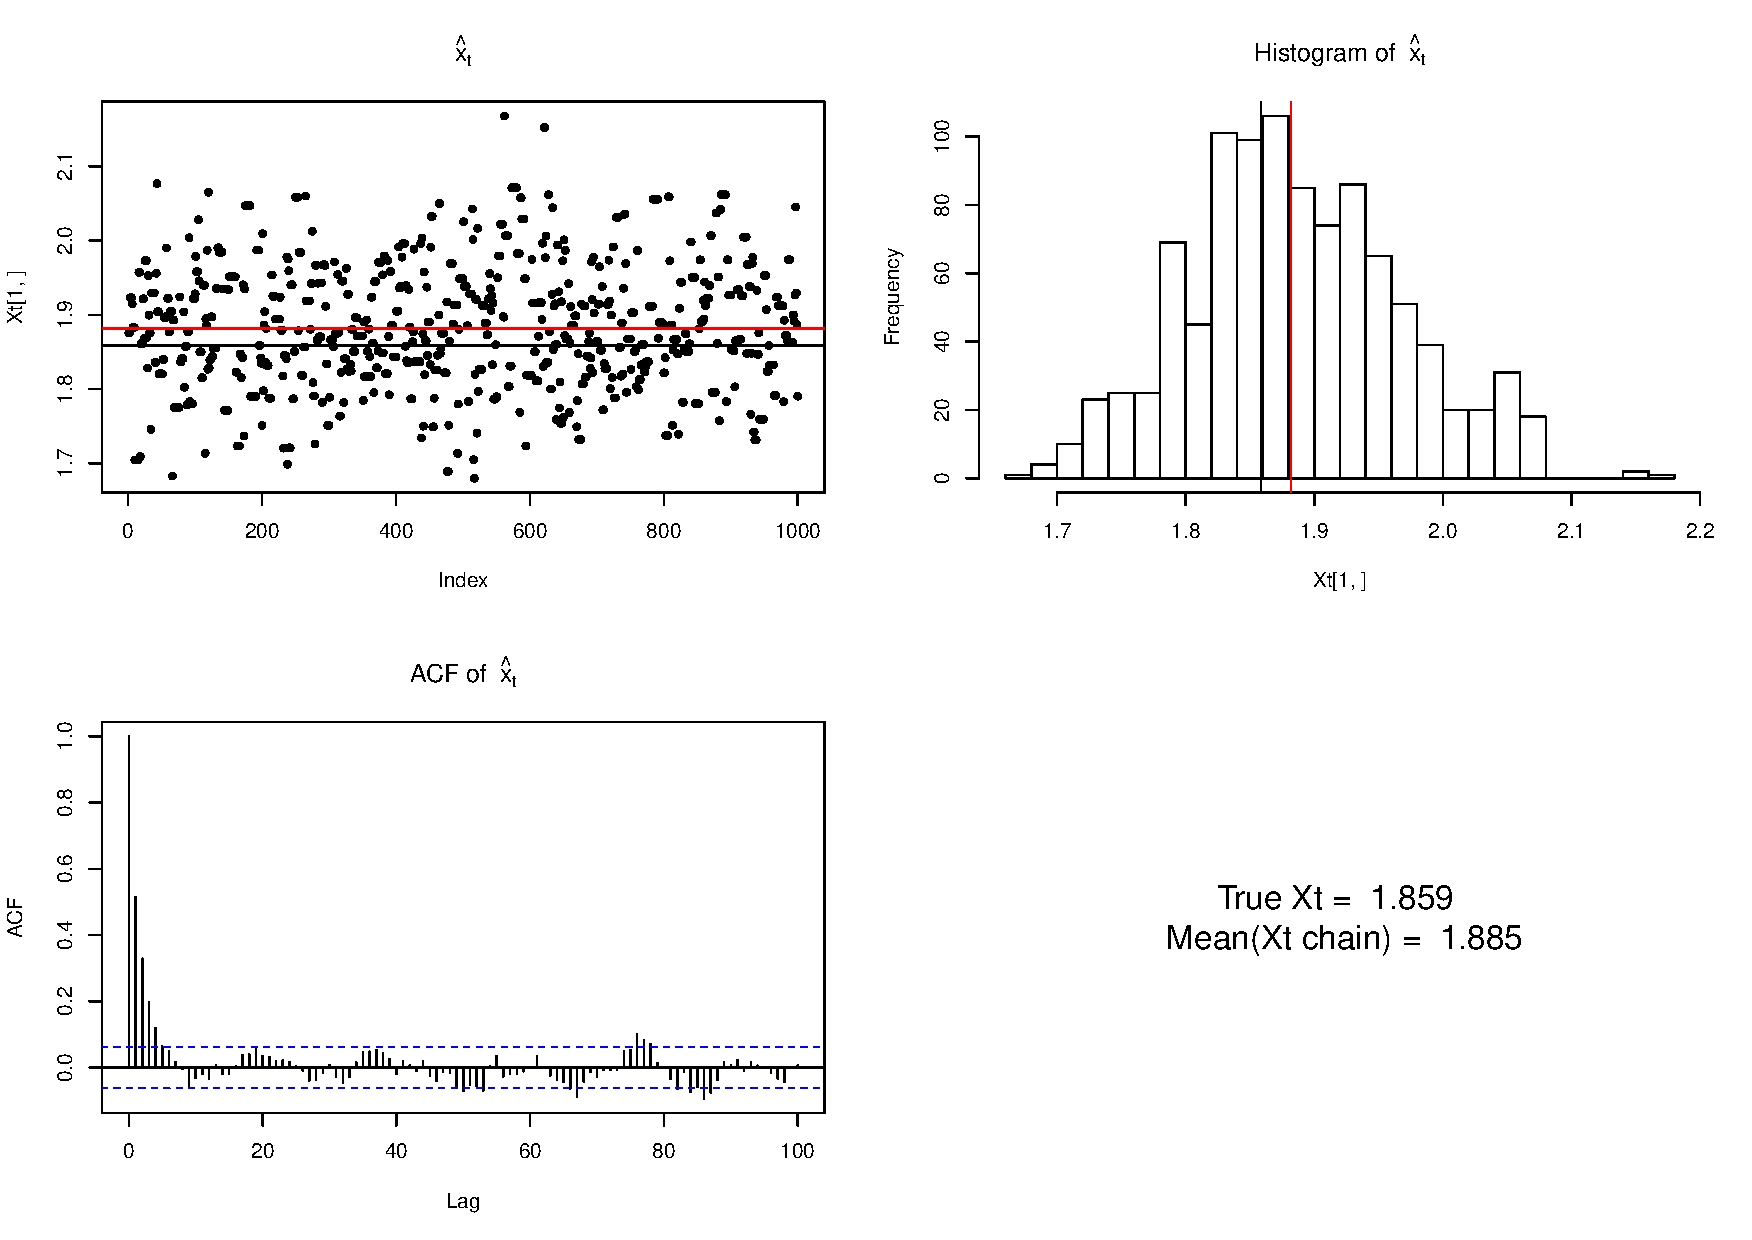
\includegraphics[width=16cm,height=10cm]{Chapters/5.MCMCOU/plots/MCMCxt}
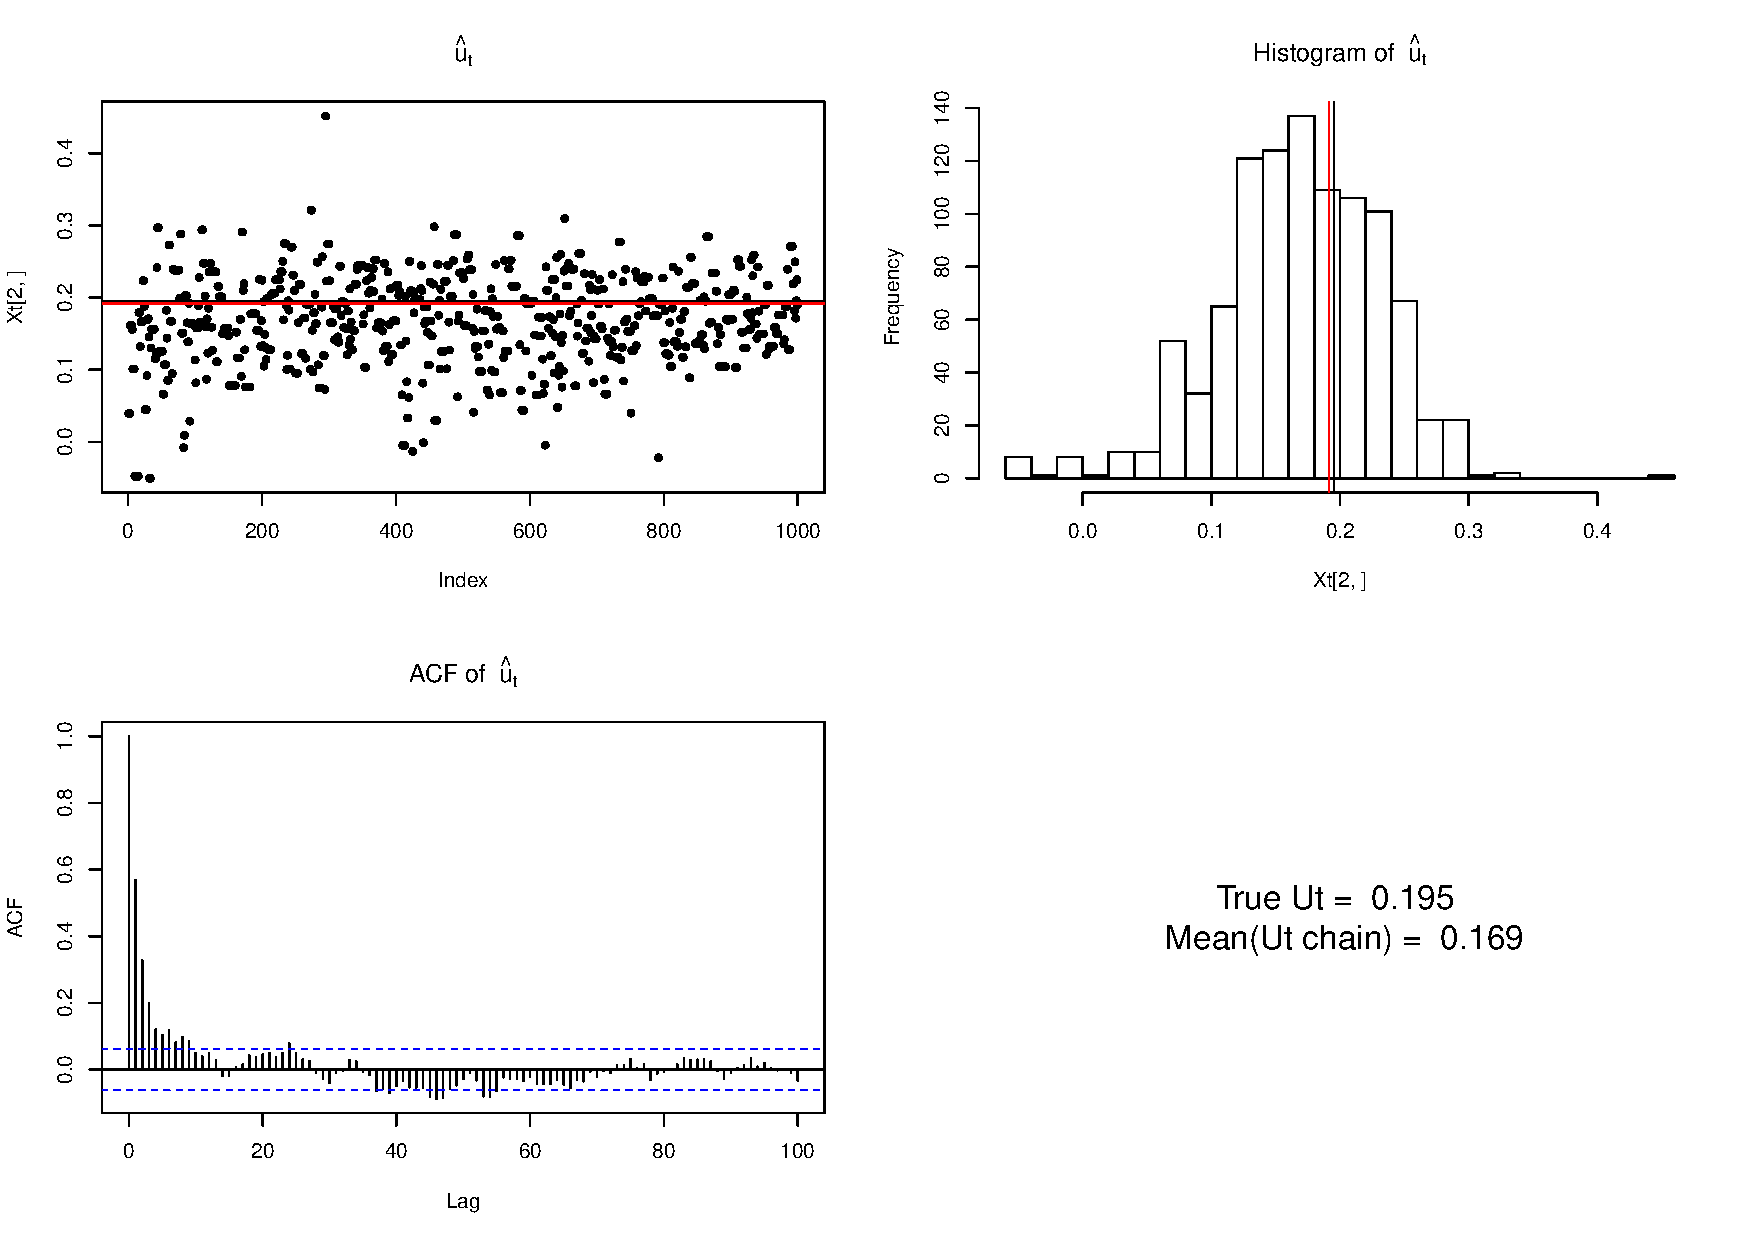
\includegraphics[width=16cm,height=10cm]{Chapters/5.MCMCOU/plots/MCMCut}
